%%%%%%%%%%%%%%%%%%%%%%%%%%%%%%%%%%%%%%%%%%  不使用 authblk 包制作标题  %%%%%%%%%%%%%%%%%%%%%%%%%%%%%%%%%%%%%%%%%%%%%%
%-------------------------------PPT Title-------------------------------------
\title{\rm{Transformer}:~自然语言处理的新范式}
%-----------------------------------------------------------------------------

%----------------------------Author & Date------------------------------------
\author[]{\vskip +10pt 姜\;\;骏\inst{}} %[]{} (optional, use only with lots of authors)
%% - Give the names in the same order as the appear in the paper.
%% - Use the \inst{?} command only if the authors have different
%%   affiliation.
\institute[BCC]{\inst{}%
%\institute[Gain~Strong]{\inst{}%
\vskip -15pt 北京市计算中心}
%\vskip -20pt {\large 格致斯创~科技}}
\date[\today] % (optional, should be abbreviation of conference name)
{	{\fontsize{6.2pt}{4.2pt}\selectfont{\textcolor{blue}{E-mail:~}\url{jiangjun@bcc.ac.cn}}}
\vskip 45 pt {\fontsize{8.2pt}{6.2pt}\selectfont{%清华大学\;\;物理系% 报告地点
	\vskip 5 pt \textrm{2025.02}}}
}

%% - Either use conference name or its abbreviation
%% - Not really information to the audience, more for people (including
%%   yourself) who are reading the slides onlin%%   yourself) who are reading the slides onlin%%   yourself) who are reading the slides onlineee
%%%%%%%%%%%%%%%%%%%%%%%%%%%%%%%%%%%%%%%%%%%%%%%%%%%%%%%%%%%%%%%%%%%%%%%%%%%%%%%%%%%%%%%%%%%%%%%%%%%%%%%%%%%%%%%%%%%%%

\subject{}
% This is only inserted into the PDF information catalog. Can be left
% out.
%\maketitle
\frame
{
%	\frametitle{\fontsize{9.5pt}{5.2pt}\selectfont{\textcolor{orange}{“高通量并发式材料计算算法与软件”年度检查}}}
\titlepage
}
%-----------------------------------------------------------------------------

%------------------------------------------------------------------------------列出全文 outline ---------------------------------------------------------------------------------
\section*{}
\frame[allowframebreaks]
{
	\frametitle{\textrm{Outline}}
%  \frametitle{\textcolor{mycolor}{\secname}}
  \tableofcontents%[current,currentsection,currentsubsection]
}
%在每个section之前列出全部Outline
%类似的在每个subsection之前列出全部Outline是\AtBeginSubsection[]
%\AtBeginSection[]
%{
%  \frame<handout:0>%[allowframebreaks]
%  {
%    \frametitle{Outline}
%%全部Outline中,本部分加亮
%    \tableofcontents[current,currentsection]
%  }
%}

%-----------------------------------------------PPT main Body------------------------------------------------------------------------------------
\small
\begin{frame}
	\frametitle{\textrm{RNN}在\textrm{NLP}中的基本思想}
    \begin{itemize}
    \item **序列建模**:~\textrm{RNN}将文本看作由单词组成的序列,通过循环结构逐词处理,每个时间步更新隐藏状态,以此保存文本的上下文信息\\
	    隐藏状态不仅受当前单词影响,还依赖之前单词的信息,借此模拟人类语言理解过程中的记忆功能
    \item **典型应用**:~在文本生成任务中,\textrm{RNN}基于已生成的单词,不断更新隐藏状态,预测下一个单词\\
	    以机器翻译为例,在将源语言翻译为目标语言时,\textrm{RNN}编码器逐词处理源语言文本,生成包含语义信息的隐藏状态;~解码器再基于这些隐藏状态,逐个生成目标语言单词
    \end{itemize}
	    \textrm{RNN}:~采用循环结构处理序列数据,每个时刻的隐藏状态不仅依赖当前输入,还依赖上一时刻的隐藏状态\\
		    这种设计使得\textrm{RNN}理论上可以捕捉长距离依赖关系,但\textrm{RNN}的循环结构决定了其计算必须按顺序进行
\end{frame}

\begin{frame}
	\frametitle{\textrm{CNN}在\textrm{NLP}中的基本思想}
    \begin{enumerate}
	    \item **局部特征提取**:~\textrm{CNN}把文本中的每个单词类比为图像中的像素,使用卷积核在文本序列上滑动,提取相邻单词组成的局部片段特征\\
		    多个不同大小的卷积核能够提取多种尺度的特征,捕捉单词间的局部语义关系
        \item **特征整合与分类**:~通过池化层对卷积得到的特征进行降维,整合局部特征,获取文本的全局特征表示,进而用于文本分类、情感分析等任务\\
		例如在情感分析中,通过卷积和池化操作提取文本特征,再经全连接层判断文本表达的情感倾向
    \end{enumerate}
	    \textrm{CNN}:~通过卷积核在数据上滑动来提取局部特征,具备平移不变性,在图像识别等领域取得了显著成果\\
		    \textrm{CNN}的感受范围通常是局部的,可以通过堆叠多层卷积来扩大感受范围
\end{frame}

\begin{frame}
	\frametitle{从神经网络到\textrm{Transformer}}
    在自然语言处理\textrm{(NLP)}和计算机视觉\textrm{(CV)}等诸多人工智能领域,循环神经网络\textrm{(RNN)}与卷积神经网络\textrm{(CNN)}曾占据主导地位,随着数据规模的增长和任务复杂度的提升,传统神经网络在长距离依赖和并行计算方面的局限性逐渐凸显
    \begin{itemize}
	    \item \textrm{RNN}:~实际训练中,由于梯度消失或梯度爆炸问题,RNN很难学习到远距离的信息,这被称为长距离依赖难题\\
		    例如:~在文本翻译任务中,开头的单词信息很难传递到句子末尾\\
		    \textrm{RNN}的循环结构无法充分利用硬件的并行计算能力,大大增加了训练时间
	    \item \textrm{CNN}通过堆叠多层卷积来扩大感受范围,获取长距离依赖信息的效率较低\\
		    比如:~在处理长文本时,难以直接捕捉到相隔较远的文本片段之间的语义关联\\
		    虽然\textrm{CNN}在一定程度上可以并行计算,但由于卷积操作的局部特性,在捕捉全局依赖关系时,计算资源的浪费较为严重
    \end{itemize}
    Transformer于\textrm{2017}年%在论文《Attention Is All You Need》中被
    提出,完全基于注意力机制,抛弃了\textrm{RNN}和\textrm{CNN}的序列结构与卷积操作,在长文本处理、并行计算上表现卓越,迅速成为\textrm{NLP}的主流模型
\end{frame}


\begin{frame}
	\frametitle{\textrm{Transformer}架构总览}
\begin{figure}[h!]
%\vspace*{-0.15in}
\centering
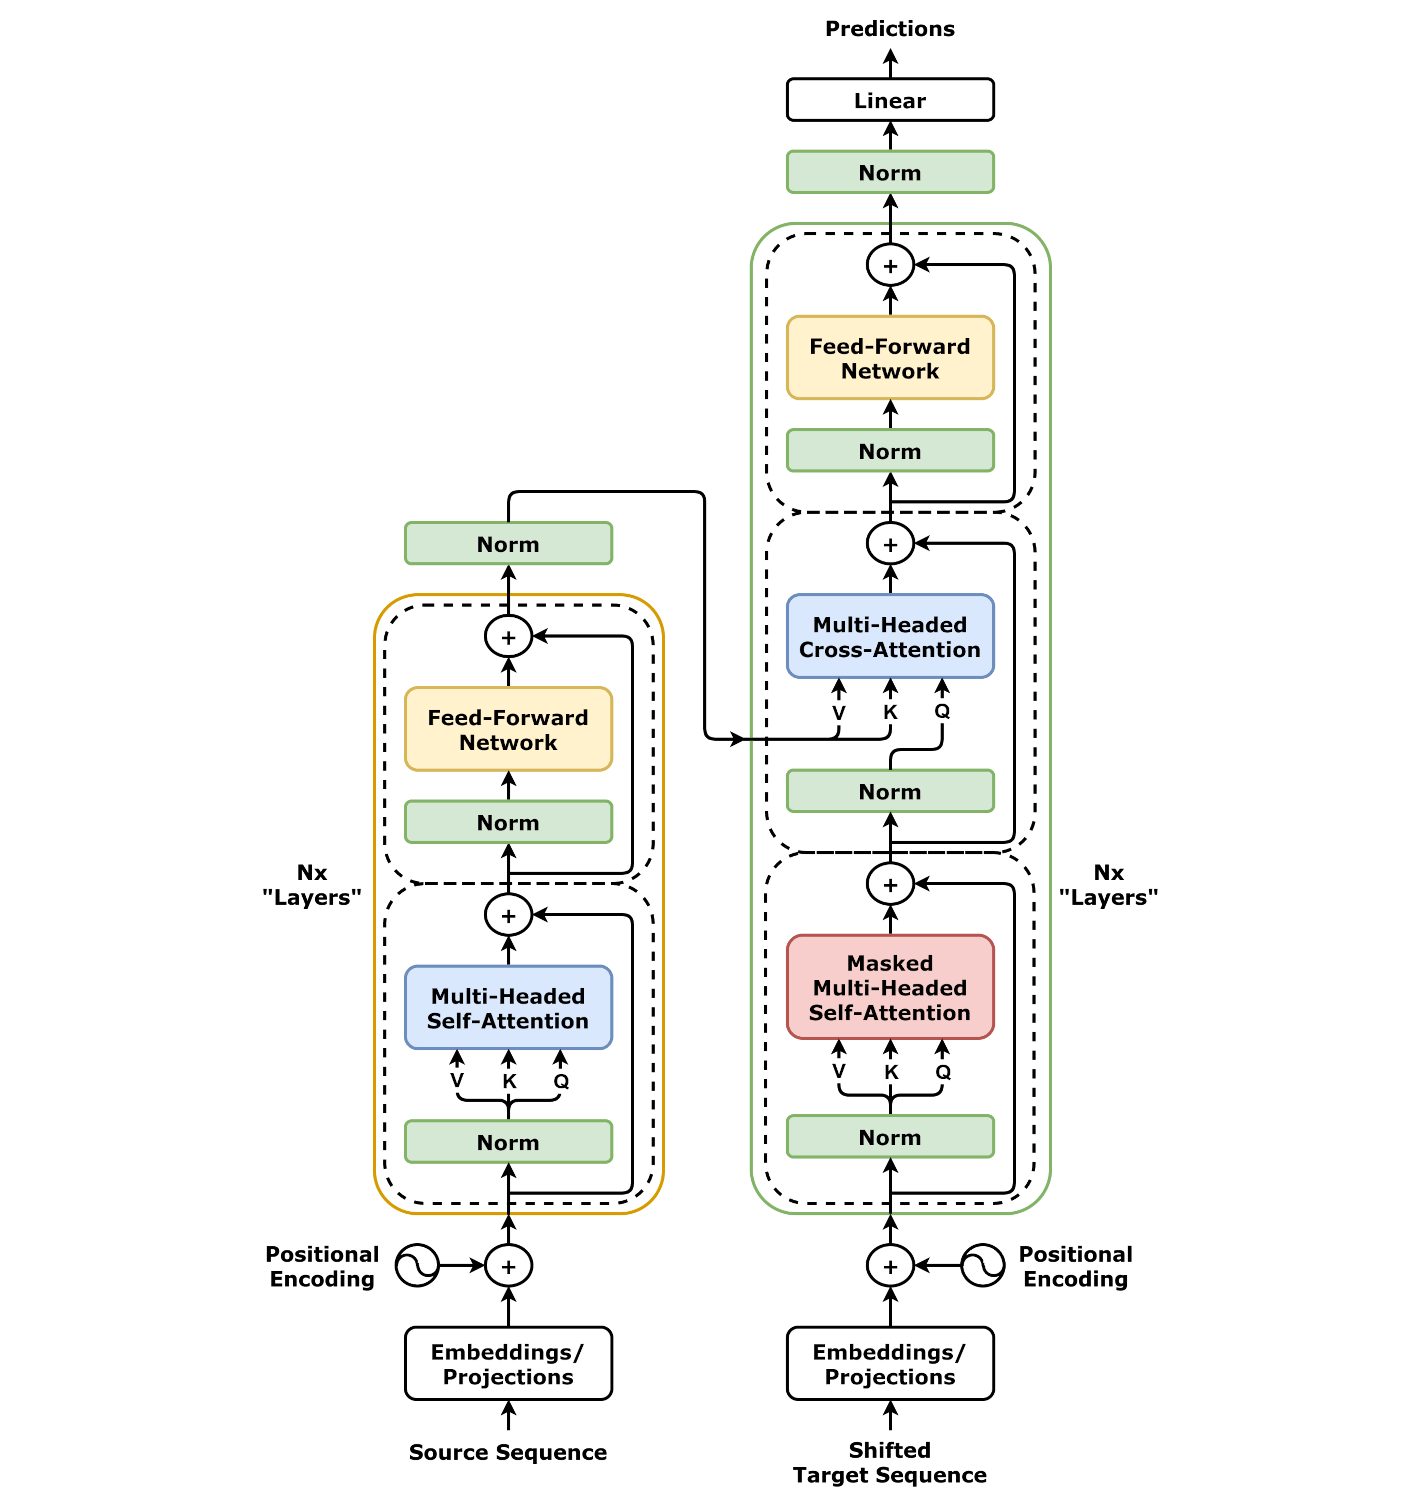
\includegraphics[height=2.2in, width=2.0in, viewport=300 0 1200 1500,clip]{Figures/Transformer_full_architecture.png}
\caption{\tiny \textrm{Transformer:~full architecture.}}%(与文献\cite{EPJB33-47_2003}图1对比)
\label{Transformer_full_architecture}
\end{figure}
    \textrm{Transformer}由编码器\textrm{(Encoder)}和解码器\textrm{(Decoder)}组成,分别包含多个相同的层,层间使用残差连接和归一化操作\\
    这些模块的设计,为并行计算提供了基础
\end{frame}

\begin{frame}
    \frametitle{并行计算:~基石模块}
    在\textrm{Transformer}中,编码器和解码器内的多个层并非按顺序逐一计算,而是可以并行处理\\
    举例来说,在编码器中每个编码器层相互独立,在计算时,所有编码器层可以同时处理输入数据的不同部分,大幅提升计算效率
\end{frame}

\begin{frame}
    \frametitle{多头注意力机制中的并行计算}
    多头注意力机制允许模型在不同的表示子空间中并行地学习相关信息
    \begin{itemize}
	    \item **计算步骤**:~输入的查询\textrm{(Query)}、键\textrm{(Key)}和值\textrm{(Value)}分别经过线性变换得到多个不同的子查询、子键和子值\\
		    由于各子查询、子键、子值的线性变换相互独立,这些操作可以并行执行\\
		    然后,计算子查询与子键的点积注意力分数,并通过\textrm{Softmax}进行归一化\\
		    最后,将加权后的子值进行拼接,并通过一个线性层得到最终的输出\\

		    用数学公式表示,对于第$i$个注意力头:~
		    \begin{displaymath}
			    \text{Attention}_i(Q, K, V) = \text{Softmax}(\frac{Q W_i^Q (K W_i^K)^T}{\sqrt{d_k}}) V W_i^V 
		    \end{displaymath}
        其中,$W_i^Q$, $W_i^K$, $W_i^V$是可学习的权重矩阵,$d_k$是键向量的维度
        \item **多注意力头整合**:~将多个注意力头的输出拼接后,再经过一个线性变换,得到最终的多头注意力输出
		\begin{displaymath}
			\text{MultiHead}(Q, K, V) = \text{Concat}(\text{Attention}_1, \ldots, \text{Attention}_h) W^O
		\end{displaymath}
        多个注意力头之间的计算过程相互独立,能够同时进行
    \end{itemize}
\end{frame}

\begin{frame}
    \frametitle{前馈神经网络中的并行计算}
    前馈神经网络在每个位置上独立运行,对注意力机制的输出进一步处理
    \begin{itemize}
	    \item **结构**:~它包含两个线性变换层,中间使用\textrm{ReLU}激活函数\\
		    数学表达式为
		    \begin{displaymath}
			     \text{FFN}(x) = \max(0, x W_1 + b_1) W_2 + b_2 
		    \end{displaymath}<++>
        其中,$W_1$, $W_2$是权重矩阵,$b_1$, $b_2$是偏置向量

	由于不同位置的输入在\textrm{FFN}中的计算彼此独立,因此可对整个序列并行计算
        \item **作用**:~为模型引入非线性变换,增强模型的表达能力,捕捉更复杂的模式
    \end{itemize}
\end{frame}

\begin{frame}
    \frametitle{解码器中的并行特性}
    解码器同样由多个解码器层堆叠而成

    与编码器不同,解码器层在多头注意力机制前多了一个掩码多头注意力机制

    虽然掩码多头注意力机制需要按顺序生成序列

    但在每个时间步内,掩码多头注意力机制与交叉注意力机制的计算,以及前馈神经网络的运算,都可以并行完成
\end{frame}

\begin{frame}
    \frametitle{掩码多头注意力机制}
    \begin{itemize}
        \item **掩码操作**:~在计算注意力分数时,通过掩码矩阵屏蔽未来位置的信息,保证模型在训练时不会“偷看”未来的输入\\
		掩码矩阵是一个上三角矩阵,对角线及以下元素为0,以上元素为负无穷,经过\textrm{Softmax}后,未来位置的注意力分数为0\\
		尽管要遵循顺序生成的原则,但在计算同一时刻的注意力分数时,各位置间的运算依然可以并行
        \item **防止信息泄露**:~这种机制确保了模型在推理过程中,只能依赖当前及之前的信息,符合自然语言处理的因果关系
    \end{itemize}
\end{frame}

\begin{frame}
    \frametitle{交叉注意力机制}
    \begin{itemize}
        \item **信息交互**:~解码器的交叉注意力机制以编码器的输出作为键和值\\
		以解码器上一层的输出作为查询,通过计算注意力分数,解码器可以从编码器的输出中获取相关的上下文信息\\
		交叉注意力机制在计算时,不同位置的查询向量与键、值向量的运算可并行进行
        \item **公式表达**:计算过程与多头注意力机制类似,只是查询、键和值的来源不同\\
		交叉注意力机制帮助解码器聚焦于输入序列的不同部分,从而更好地生成输出
    \end{itemize}
\end{frame}

\begin{frame}
	\frametitle{与\textrm{RNN}、\textrm{CNN}的对比}
    \begin{table}[ht]
        \centering
        \begin{tabular}{|l|l|l|}
            \hline
	    特性 & \textrm{RNN} & \textrm{Transformer} \\
            \hline
            结构 & 循环结构,顺序处理数据 & 并行处理数据 \\
            \hline
            长距离依赖 & 梯度消失或爆炸,难以处理长距离依赖 & 自注意力机制,有效捕捉长距离依赖 \\
            \hline
            计算效率 & 顺序计算,效率低 & 并行计算,效率高 \\
            \hline
        \end{tabular}
	\caption{\textrm{RNN}与\textrm{Transformer}的对比}
    \end{table}
    \begin{table}[ht]
        \centering
        \begin{tabular}{|l|l|l|}
            \hline
	    特性 & \textrm{CNN} & \textrm{Transformer} \\
            \hline
            感受野 & 局部感受野,通过堆叠扩大感受野 & 全局感受野,自注意力机制获取全局信息 \\
            \hline
            归纳偏置 & 平移不变性,局部连接 & 无特定归纳偏置 \\
            \hline
            应用场景 & 图像领域表现出色 & NLP领域表现出色 \\
            \hline
        \end{tabular}
	\caption{\textrm{CNN}与\textrm{Transformer}的对比}
    \end{table}
\end{frame}

\begin{frame}
    \frametitle{总结}
    \textrm{Transformer}凭借自注意力机制和精心设计的架构,实现了高效的并行计算,解决了长距离依赖和并行计算的问题,在\textrm{NLP}领域取得了巨大成功\\

    它不仅革新了\textrm{NLP}研究,也推动了其他领域如计算机视觉的发展,未来有望在更多领域发挥重要作用
\end{frame}
